\section{Use Cases}
\labsec{ch04-use-cases}

The first stage to analyze our system is to see the use cases view, from there we will try to capture posible requirements and with all that information design our system.

\begin{figure}[hb]
    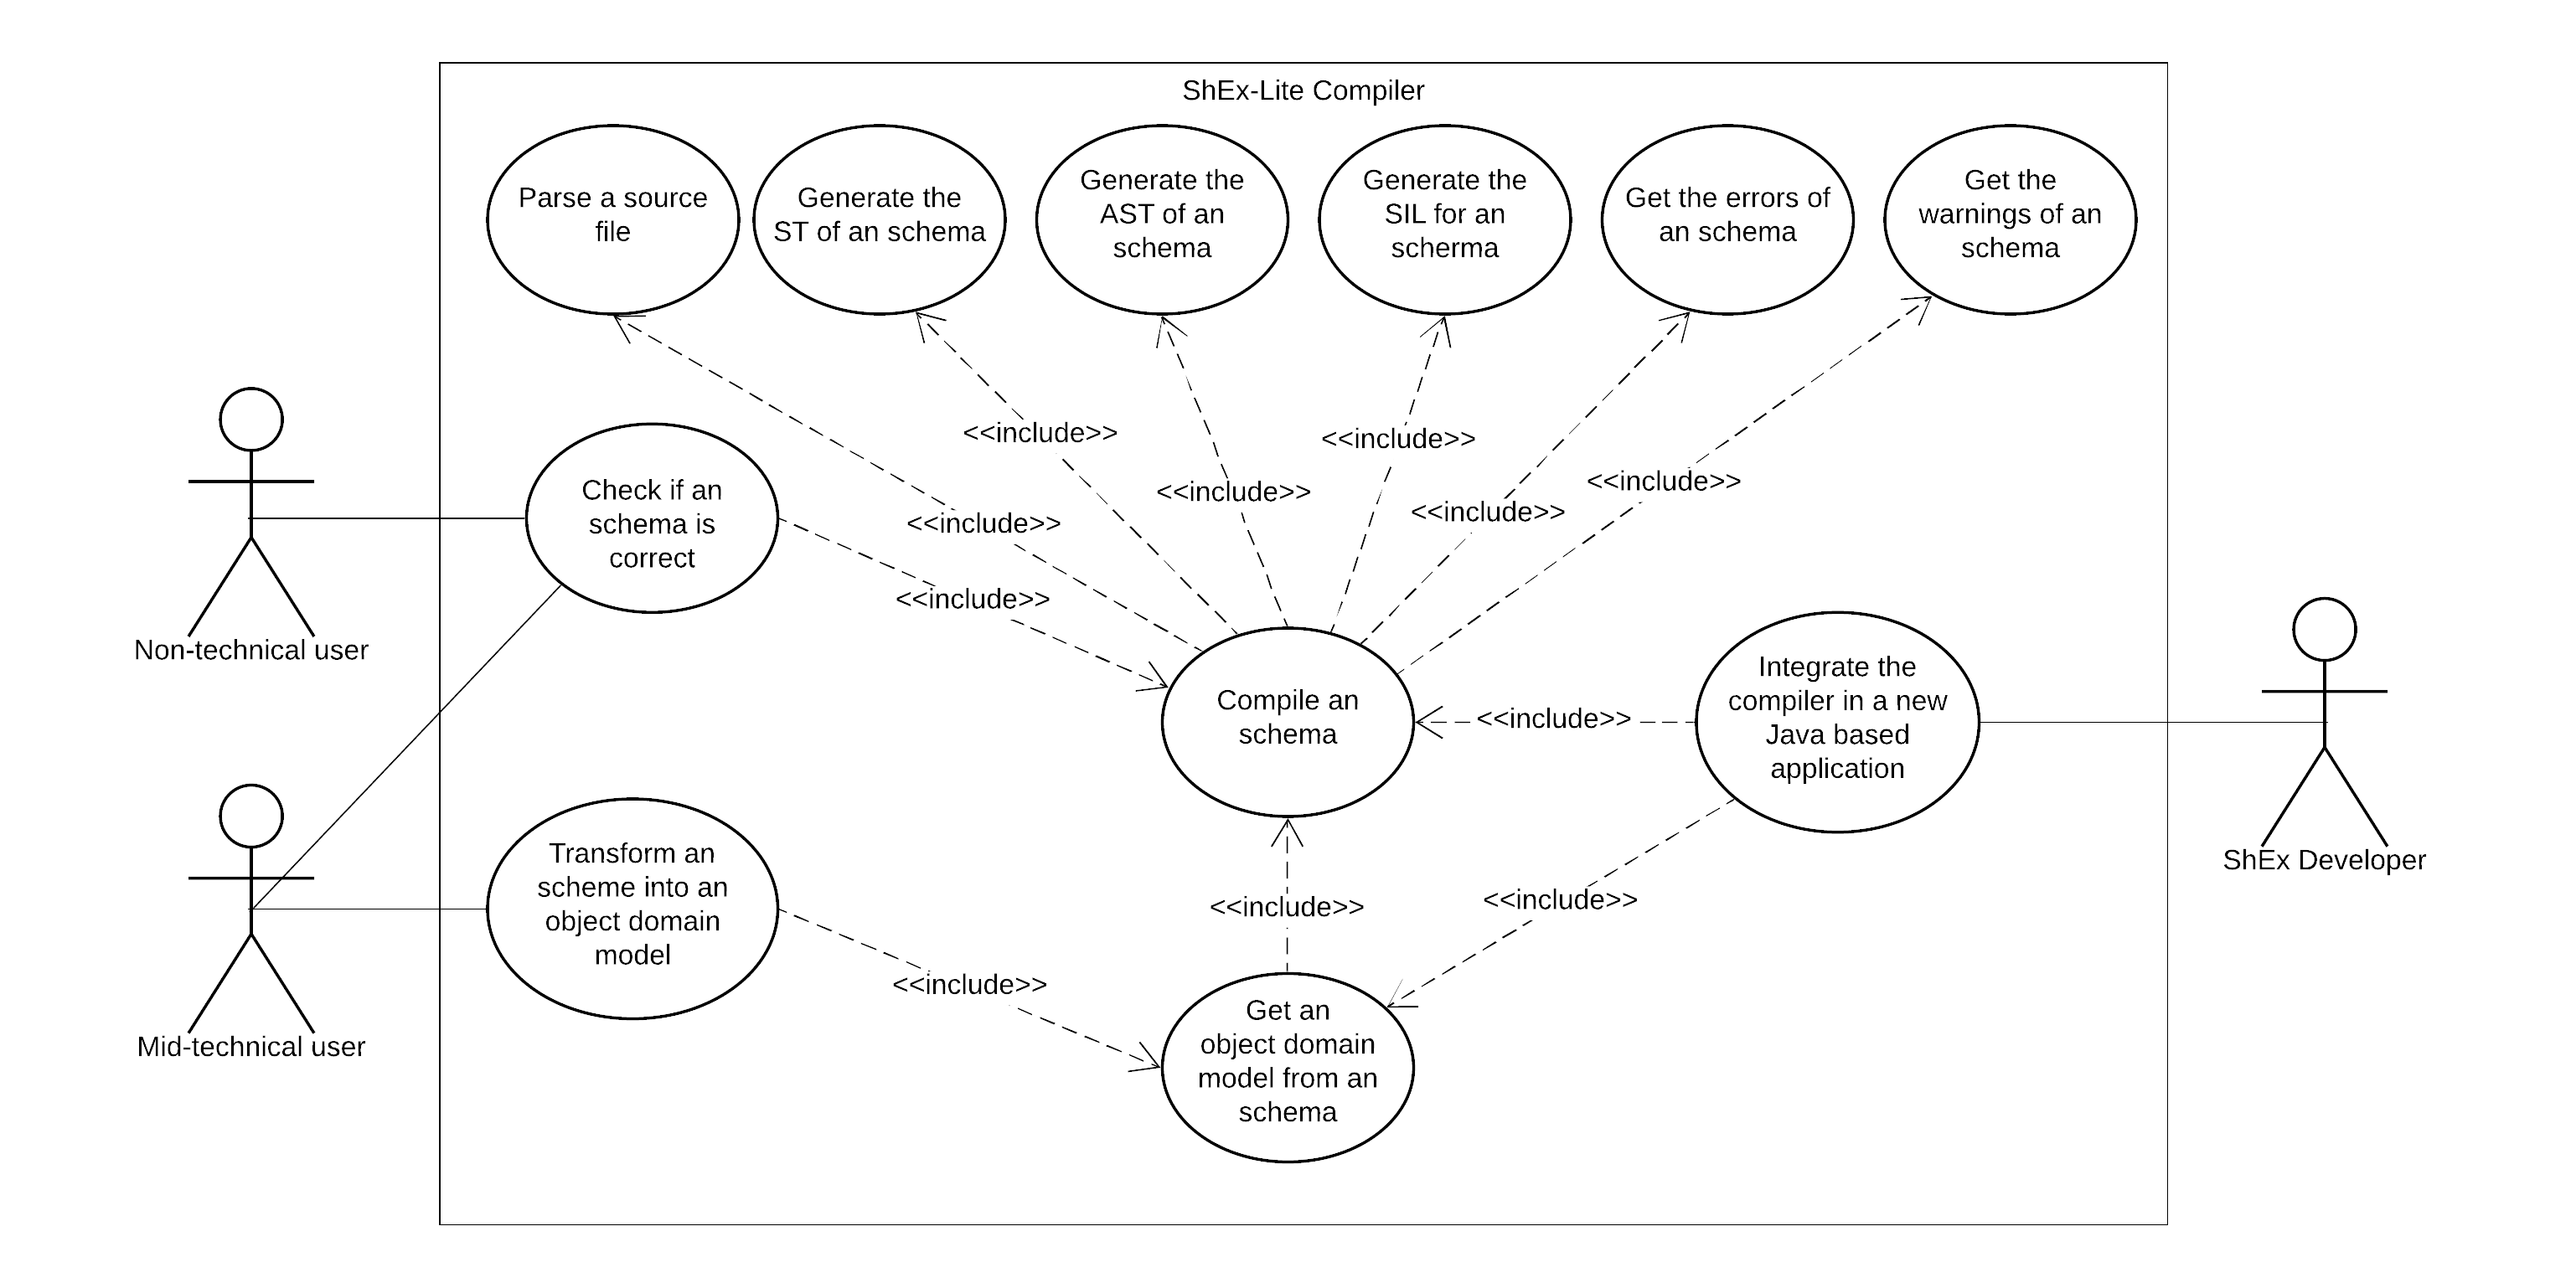
\includegraphics{shex-lite-use-cases-01.png}
    \caption[Use cases view of the ShEx-Lite compiler for the three different actors of the system]{Use cases view of the ShEx-Lite compiler for the three different actors of the system.}
    \labfig{shex-lite-use-cases-01}
\end{figure}

In \reffig{shex-lite-use-cases-01} we can see the high level view of the different use cases that the three different target users of the systems might have, now we will analyze each one individually, some the internal use cases that have no direct interaction with the target user will be explored after.

\subsection{Non technical user}
The non technical target user is intended to use only the compiler to validate if the schemas they have defined are syntactically and semantically correct, or if they have any error or warning to be aware of them. \reffig{shex-lite-use-cases-02} shows the interaction diagram for this actor, and \reftab{use-case-01-tab} describes the represented use case.

\begin{figure}[hb]
    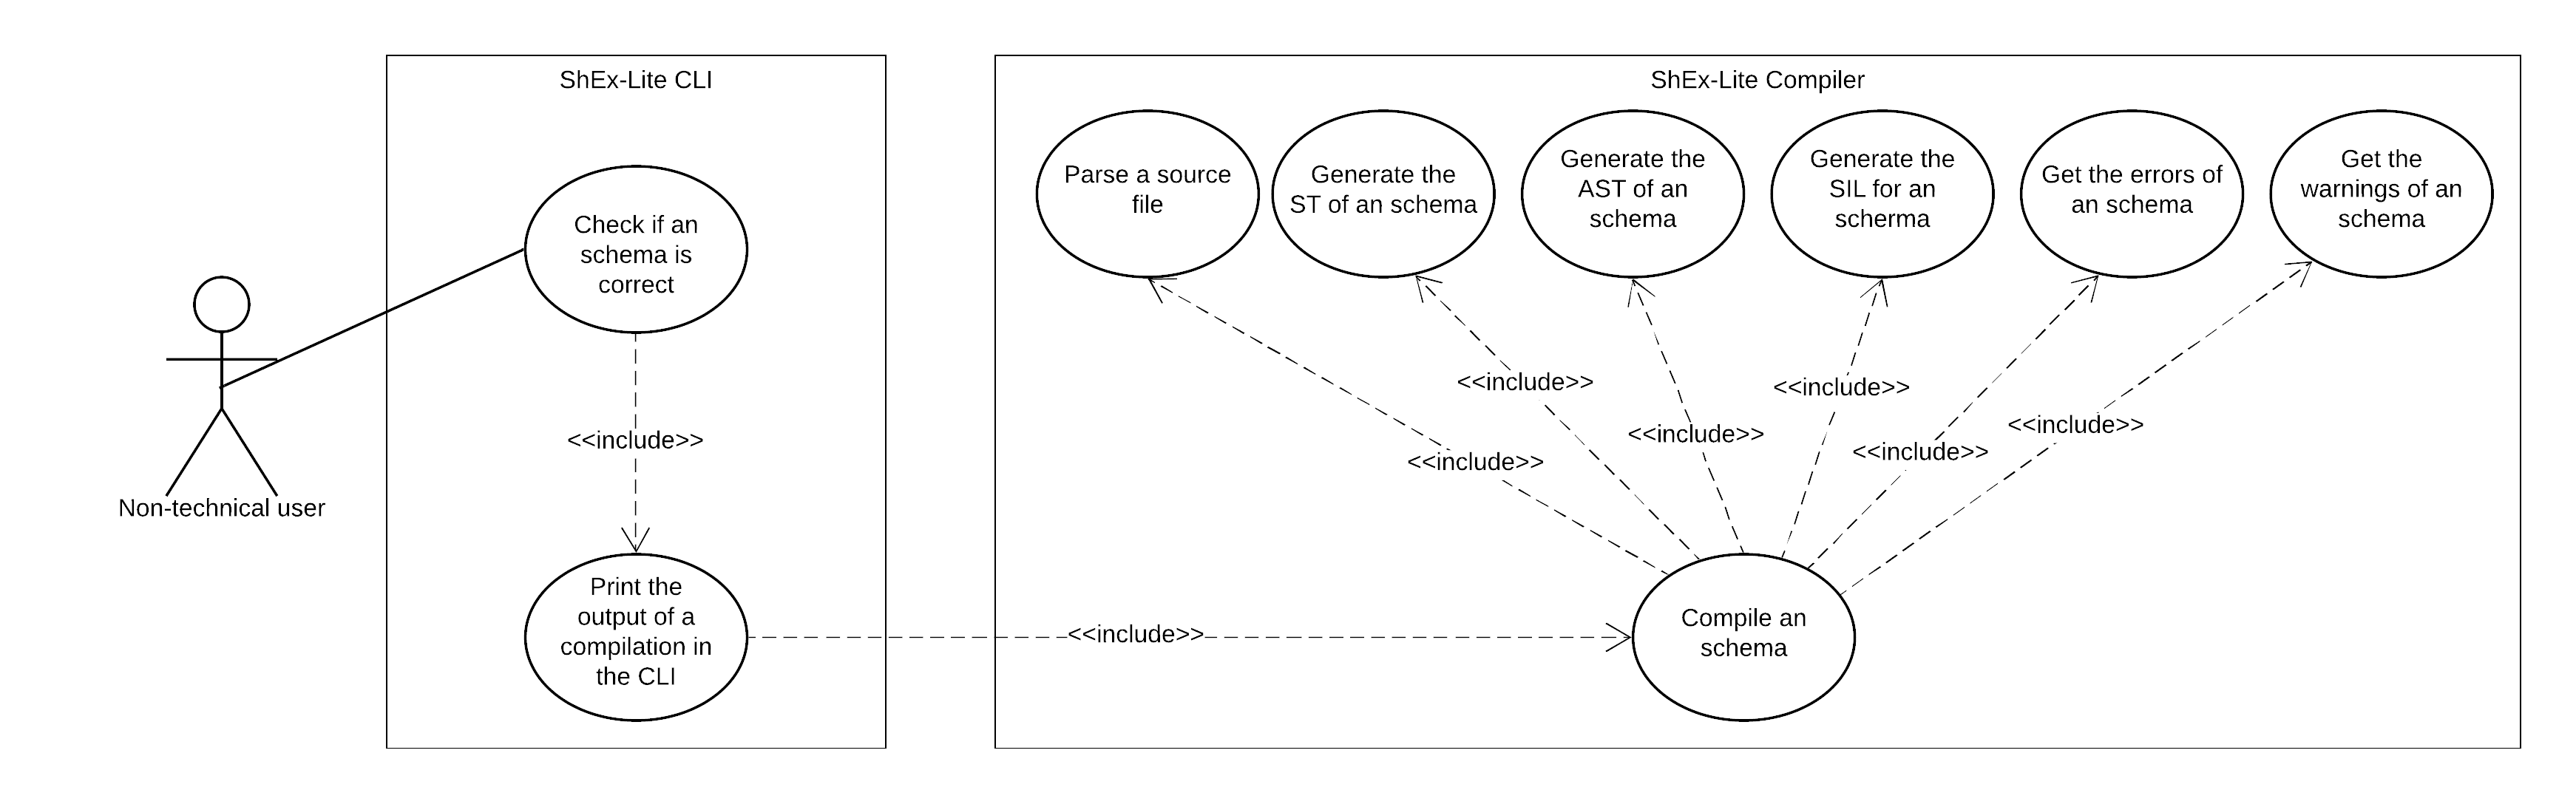
\includegraphics{shex-lite-use-cases-02.png}
    \caption[Extension of the use case view for a non technical user]{Extension of the use case view for a non technical user.}
    \labfig{shex-lite-use-cases-02}
\end{figure}

\begin{table}
    \begin{tabular}{ | m{2cm} | m{8cm}| }
        \toprule
        Use Case Number & 1 \\
        \midrule
        Description & Check if an schema is correct from the CLI tool. \\
        \midrule
        Actor & Non technical user. \\
        \midrule
        Flow & The actor wants to check if schema is correct or not. If it is not correct wants to see all the warnings / errors. For this purpose the actor introduces the schema in the CLI tool and starts the flow. Once the flow is complete the actor wants to see information that helps to decide if the schema is correct or not. \\
        \bottomrule
    \end{tabular}
    \caption[Definition of the use case number 1 for the non technical user]{Definition of the use case number 1 for the non technical user.}
    \labtab{use-case-01-tab}
\end{table}

\subsection{Mid technical user}
The use cases expected for a mid technical user are two, in one side the compilation in order to validate if their schemas are syntactically and semantically correct, or if they have any error or warning. And on the other hand, automatically generate the domain object models for the defined schema. For this user we can find the representation of the interaction diagram at \reffig{shex-lite-use-cases-03} and both associated use cases descriptions on \reftab{use-case-02-tab} and \reftab{use-case-03-tab}.

\begin{figure}[hb]
    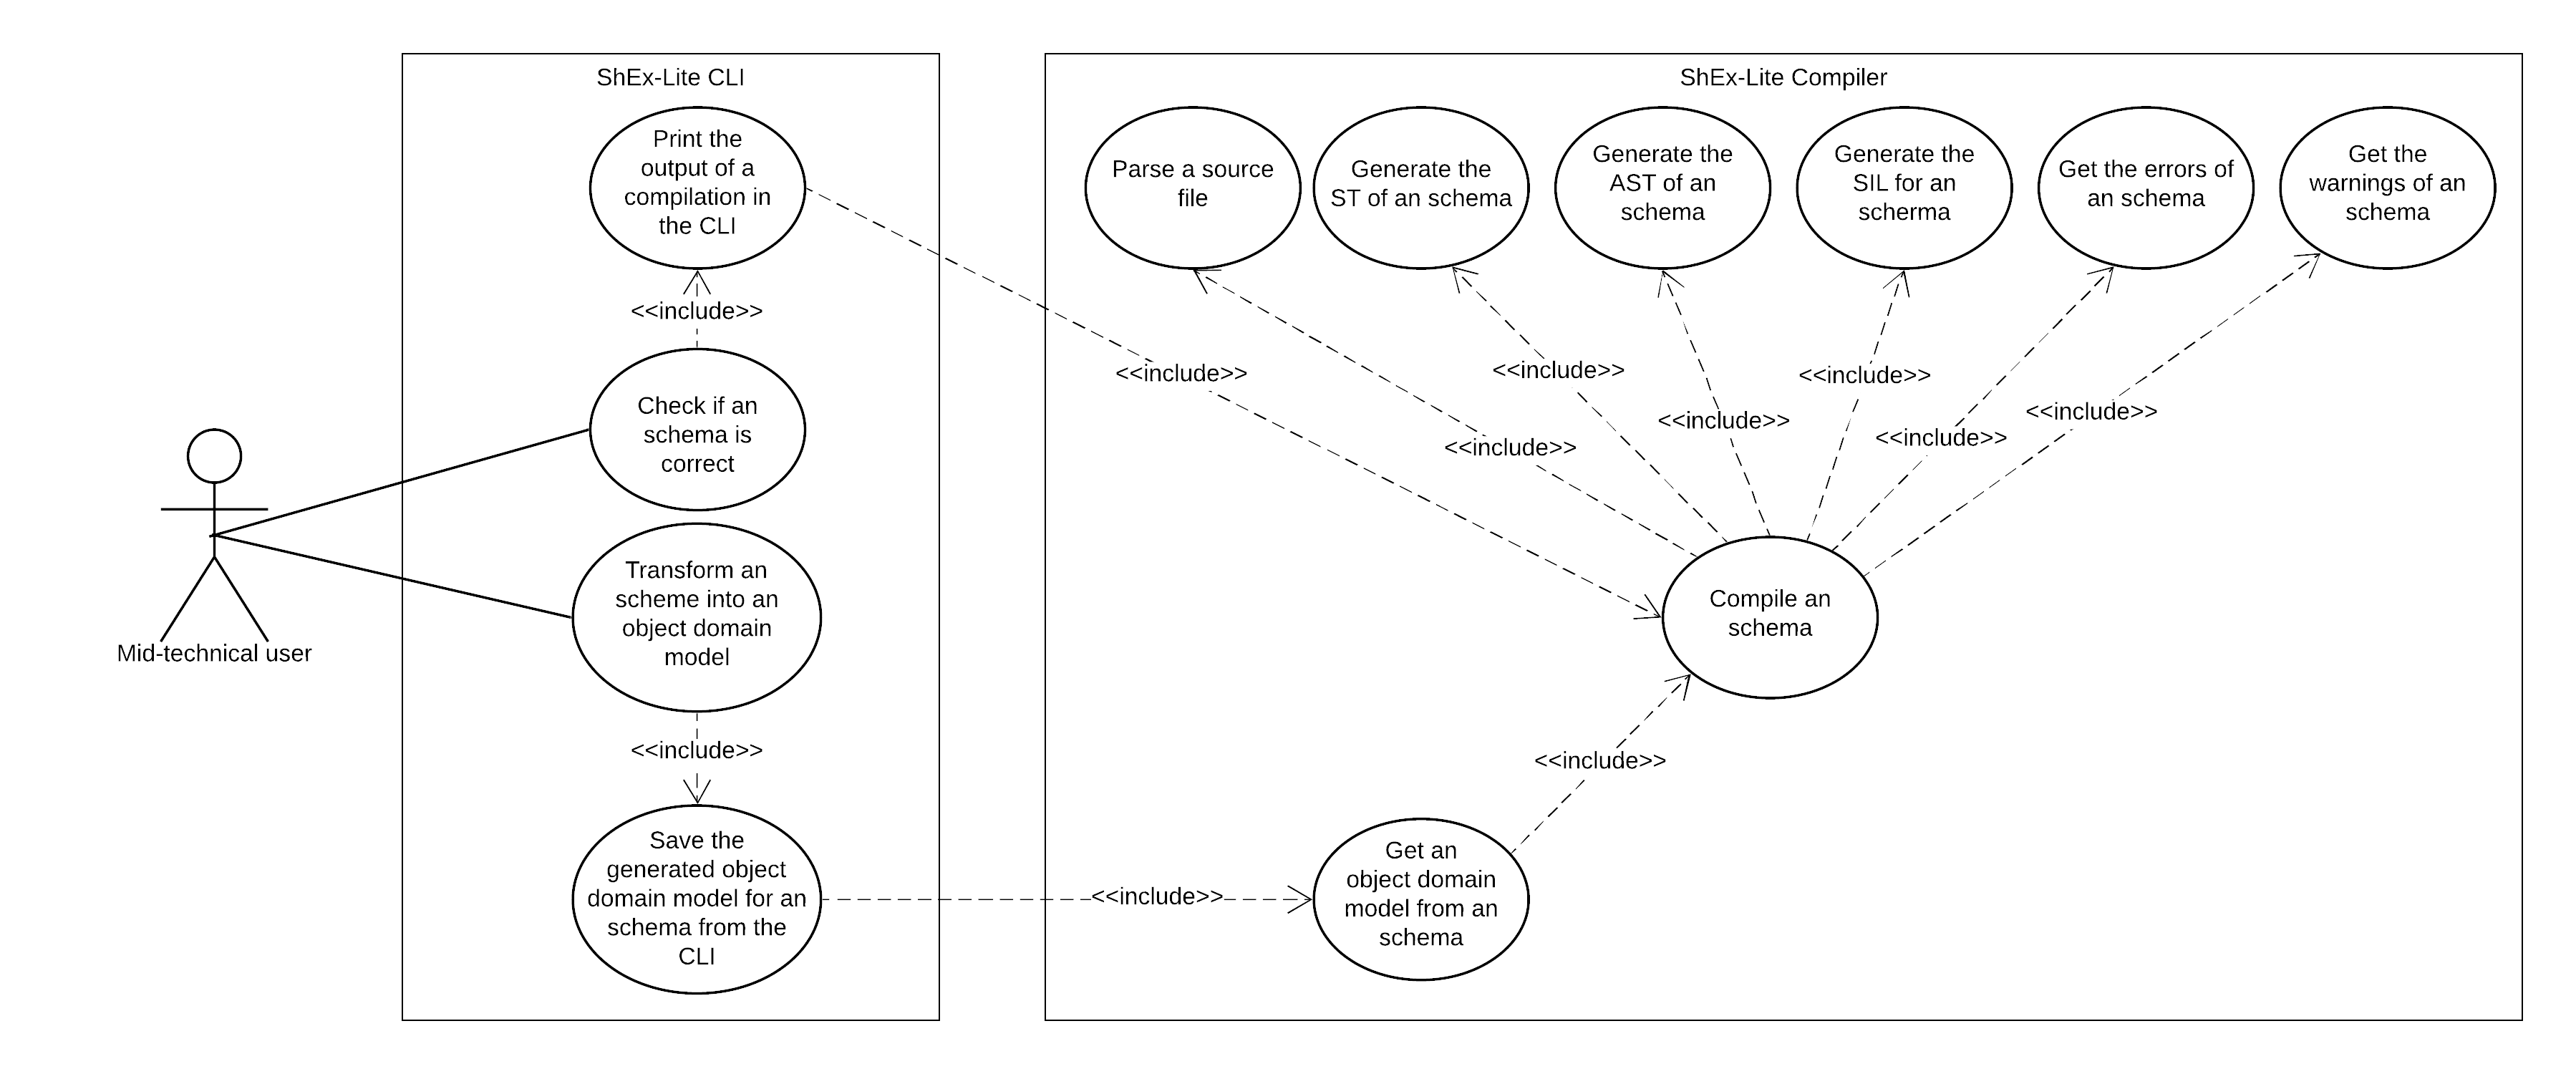
\includegraphics{shex-lite-use-cases-03.png}
    \caption[Extension of the use case view for a mid technical user]{Extension of the use case view for a mid technical user.}
    \labfig{shex-lite-use-cases-03}
\end{figure}

\begin{table}
    \begin{tabular}{ | m{2cm} | m{8cm}| }
        \toprule
        Use Case Number & 2 \\
        \midrule
        Description & Generate an object domain model for a given schema from the CLI. \\
        \midrule
        Actor & Mid technical user. \\
        \midrule
        Flow & The actor wants to generate an object domain model for a given schema from the CLI tool. For this purpose the actor introduces the schema in the CLI tool and starts the flow. Once the flow in complete the actor wants the generated object model to be persist as source files on his computer. \\
        Conditions & For this flow to end correctly it is mandatory that the schema that the user uses to generate the domain object model is correct. \\
        \bottomrule
    \end{tabular}
    \caption[Definition of the use case number 2 for the mid technical user]{Definition of the use case number 2 for the mid technical user.}
    \labtab{use-case-02-tab}
\end{table}

\begin{table}
    \begin{tabular}{ | m{2cm} | m{8cm}| }
        \toprule
        Use Case Number & 3 \\
        \midrule
        Description & Check if an schema is correct from the CLI tool. \\
        \midrule
        Actor & Mid technical user. \\
        \midrule
        Flow & The actor wants to check if schema is correct or not. If it is not correct wants to see all the warnings / errors. For this purpose the actor introduces the schema in the CLI tool and starts the flow. Once the flow is complete the actor wants to see information that helps to decide if the schema is correct or not. \\
        \bottomrule
    \end{tabular}
    \caption[Definition of the use case number 3 for the mid technical user]{Definition of the use case number 3 for the mid technical user.}
    \labtab{use-case-03-tab}
\end{table}

\subsection{ShEx Developer}
A ShEx developer is expected to use the compiler in two ways, first to integrate it in to other applications and secondly to generate object domain models for a given schema but not from the CLI, from an API instead. \reffig{shex-lite-use-cases-04} shows the interaction diagram of this actor with the compiler and \reftab{use-case-04-tab} descrives this use case scenario.

\begin{figure}[hb]
    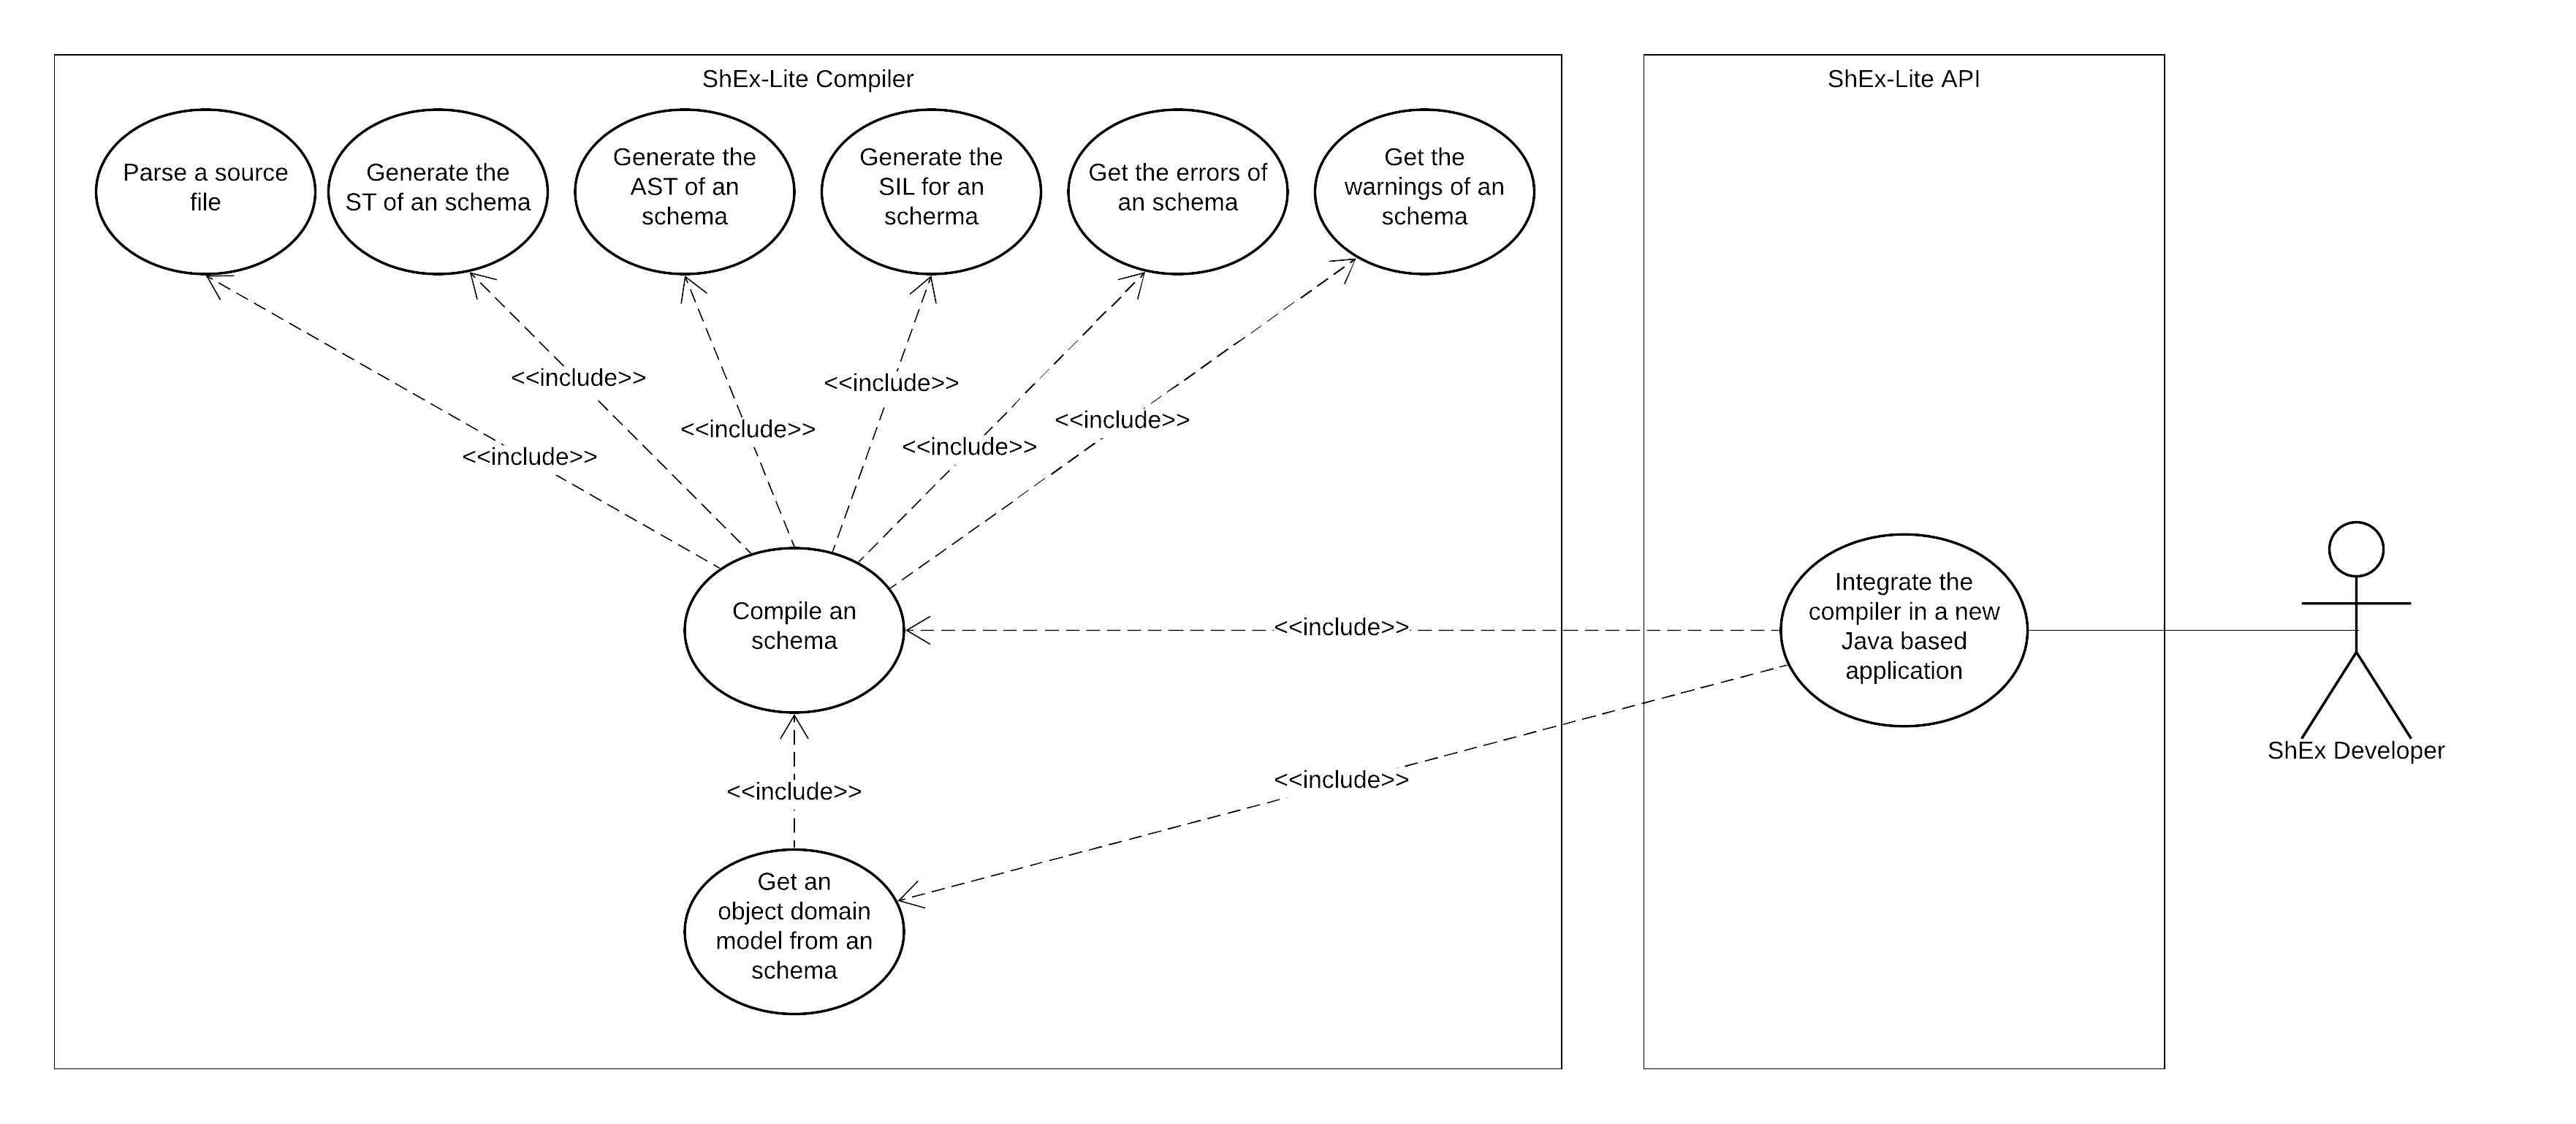
\includegraphics{shex-lite-use-cases-04.png}
    \caption[Extension of the use case view for a mid technical user]{Extension of the use case view for a mid technical user.}
    \labfig{shex-lite-use-cases-04}
\end{figure}

\begin{table}
    \begin{tabular}{ | m{2cm} | m{8cm}| }
        \toprule
        Use Case Number & 4 \\
        \midrule
        Description & Integrate the compiler in a new Java based application. \\
        \midrule
        Actor & ShEx developer. \\
        \midrule
        Flow & The actor wants to integrate the compiler in to a new java base application. For that purpose the actor will use a public API that allow the actor to integrate the actions described in the use cases 2 and 3. \\
        \bottomrule
    \end{tabular}
    \caption[Definition of the use case number 4 for the ShEx developer user]{Definition of the use case number 4 for the ShEx developer user.}
    \labtab{use-case-04-tab}
\end{table}

\bigskip
The previous use cases might seem like the system is really simple, but far from truth the
fact that the interface with the target users is simple does not define the complexity of the
system, as this, lives inside of it. In order to capture this complexity we will proceed now to
analyze the requirements that the implemented system must meet. 